%*******************************************************************************
%*********************************** First Chapter *****************************
%*******************************************************************************

\chapter{Introduction} \label{ch:Introduction} %Title of the First Chapter

\ifpdf
    \graphicspath{{Chapter1/Figs/Raster/}{Chapter1/Figs/PDF/}{Chapter1/Figs/}}
\else
    \graphicspath{{Chapter1/Figs/Vector/}{Chapter1/Figs/}}
\fi


%********************************** %First Section  **************************************
\section{System Biology}
The prime goal of Biology is to get the insight of various principle and detail of biological systems. More than six decade ago, Watson and Crick discover the structure of DNA (\cite{Watson:1953}) and radically changed the way of study and development of biology and biological systems. They explained the biological phenomena with the help of molecular basis. This new concept help to explain different aspect of biology like heredity, different disease, various evolutionary aspects as well as development with more firm theoretical ground. Since then, biology became a framework of knowledge governed by some basic and fundamental laws of physics.

Due to the enormous advancement of molecular biology, at present we have in-depth knowledge of elementary processes like evolution, heredity, disease, development etc. These mechanisms also includes other biological features like replication, transcription, translation, and so on. Accomplishment of symbolic DNA sequencing helped to reveal large number of genes and their transcriptional products. DNA sequences for many organisms like \textit{Mycoplasma, Plasmodium falciparum, Saccharomyces cerevisiae, \textit{Caenorhabditis elegans}, Drosophila melanogaster, Homo sapiens} and many more have been fully identified. Due to the advancement of different methods gene expression profile are available at the mRNA level. Even measurement of protein level and their different subsequent actions are also making progress. 

Undoubtedly understanding at the molecular level will accelerate to understand the biological systems but these knowledge isn't sufficient to understand biological systems as systems. Genes and protein are few components of a whole system. It is necessary to understand what constitute the system, but even only this knowledge is not sufficient to understand the complete system. System biology is a new field of biology to acquire understanding up to system level of biological system (\cite{Kitano:2000}). 

The extent of the area of system biology is very broad and various technique may be may be required for each individual research target. Very often it demands combined effort from multiple discipline research area like molecular biology, high-precision measurement technology, mathematics, computer science, control theory and other engineering and scientific field. \cite{Kitano:2002} mentioned the main four key areas to carried out the research: $(1)$ genomic and other molecular biology research, $(2)$ various technology for comprehensive and high-precision measurements, $(3)$ computational studies, such as bioinformatics, modelling and simulation, software tools, and $(4)$ analysis of the dynamics of the systems. This clearly depicts requirement of multi-disciplinary research effort to get the knowledge of biological systems as systems. The abstract concept of system yet more than a collection of multi-disciplinary research components. To obtain the proper insight of system beside the detail description of the components it is also essential to know what happens during the period or processes when any stimuli and/or disruptions take place.

Identification of the system structure is the primary requirement to understand biological system. Some of the key structure might be different regulatory relationship of genes and interactions with protein that shows the metabolism pathway and signal transduction, physical structure of chromatin, cells, organisms and other components. Though it is very critical to monitor biological processes in bulk using high-throughput DNA micro-array, real-time polymerase chain reaction (RT-PCR), protein chips and other methods thereafter methods to identify genes and metabolism network have to be established. Once a system structure is established up to a certain degree, it is required to find out the behaviour. To understand the behaviour properly a number of analysis method can be used. For example, if we want
to know the sensitivity of a specified behaviour against some external perturbations, and its time to return its normal state since the stimuli take place. This type of analysis provides the system level characteristics as well as uncover important insights of medical treatments by revealing cell response to certain chemical affinities. 

To apply the knowledge obtained from system structure and behaviour understanding, further research is required to control the state of the biological systems. All these phases leads toward the establishment of technologies those allow us to design biological system which can provide cures for different diseases. Even some futuristic example could be organ cloning technique for the treatment of diseases what require organ transplants or building biological materials for engineering specially robotics having self-sustaining and self-repairing capabilities.

\section{Dynamic Mathematical model: what and why in System biology?}
Any models are abstractions of reality. Models mostly designed to focus of specific aspects of the objects for certain kind of study. usually other aspects are abstracted away. Biologists almost regularly making use of tangible 'real world' models. Some of them are very simple like molecular ball-and-stick, again some of them are complex such as animal disease model or model organisms. They also use 'conceptual models'. These conceptual models usually take the form of verbal descriptions of the system and communicate by diagrams. These diagrams are usually constructed with a set of components and the ways they interact with each other. While representing knowledge of cellular or different other processes, these interaction diagrams, or 'cartoon' models may play a central role (\cite{Ingalls:2012}).

\begin{figure}%[b]
	\centering
		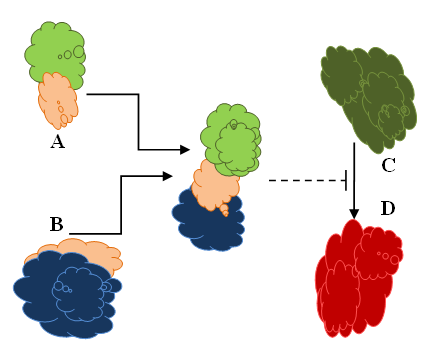
\includegraphics[scale=.45]{ProtienProtien.png}
		\rule{35em}{0.5pt}
	\caption[A ‘cartoon’ model of protein protein interaction.]{A ‘cartoon’ model of protein protein interaction. Two different molecular species A and B bind to form a complex molecular. The newly formed complex hinder the rate at which molecules of species C are transformed to species D.}
	\label{fig:Protein protein interaction}
\end{figure}

A major drawback of these cartoon models is that while considering system behaviour they could be significantly ambiguous. It even more, if there is any interaction network related with feedback. Complexity increases even further when the number of components and their corresponding interactions in the network grows. Sometimes it become very difficult to get the intuitive understanding of the system behaviour. But a mathematical model or description of the same model can eliminate uncertainty of the model behaviour. The mathematical model will consider the quantitative representation of individual interaction of the cartoon model. In Figure \ref{fig:Protein protein interaction} species A and B bind to form a new complex. The newly formed complex hinder the rate at which molecules of species C are transformed to species D. A numerical description of the process is required to quantify the interaction. Though for simple cases only equilibrium condition is enough, but in many other cases binding and unbinding rates might be also required. The cartoon model or traditional knowledge cannot provide a quantitative description rather a qualitative explanation of the molecular interaction. But a well studied mechanisms with sufficient data might be capable to show the quantitative characteristics. The interaction diagram with related quantitative data can be used to develop a dynamic mathematical model. This kind of model consists a number of equations that describe the systems behaviour over time. This behaviour is termed as ``system's dynamic behaviour''. These models are usually \textit{mechanistic}, as they explain the mechanisms of molecular interaction with some laws of physics and chemistry as well as mathematics. Any of the part of the mechanistic model actually represent the real observed system. Any change in the mechanistic model's component will also mimic to the real system. So, model simulation (\textit{in silico} experiments) can be used to predict system behaviour. Some numerical software built with different programming language are used for this simulation purposes. 

As mathematical model is a hypothesis, so the outcome or result of the model hypothesis are also hypothesis. Though the real cellular behaviour definitively cannot predict by simulation, but they can be invaluable for further experimental design by showing the promising paths for further investigation, or by showing the inconsistencies between the real laboratory observations and our understanding about the model or system. 

\section{The Systeome Project}
"Systeome" is an collection of system profile for all genetic variations and environmental stimuli response. A system profile consists of a set of information about the properties of the system including structure, behaviour, analysis of result such as bifurcation diagram or phase portfolio. The structure of the system should include structure of gene and metabolic networks and its physical structure, associated constants, and their properties (\cite{Kitano:2002}).

Systeome is not just a simple cascade map rather it assumes different active and dynamic solutions, simulations as well as profiling of various system status. The Systeome project might be established with dealing all aspects for profiling the Systeome of yeast, \textit{C. elegans, Drosophila,} mouse and finally human. The primary goal of the Human Systeome project is defined as- ``To complete a detailed and comprehensive simulation model of the human cell at an estimated error margin of 20 percent by the year 2020, and to finish identifying the system profile for all genetic variations, drug responses, and environmental stimuli by the year 2030''(\cite{Kitano:2002}).

This is a highly ambitious project, and requires several milestones. Some pilot projects will lead toward the final goal. Initial pilot projects are using yeast for the simplicity of structure and subsequent behaviour. \textit{C.elegans} have comparatively complex system structure and so is their behaviour. Beside such pilot projects concurrently the Human Systeome project shall be commenced.

The futuristic impact of this project will be very wide spread as well as far-reaching. These will be the baseline and standard asset for any further biological research to provide fundamental diagnostics and prediction for a variety of medical practice. This Systeome project involves many other major engineering projects for developing the measurements, as well as software platform.

\section{Biological Background}
In modern molecular biology the biological systems like cells are treated as a complex systems. The usual conception of the complex system is a very large number of simple but identical elements interact to generate the complex behaviour. But the actual behaviour of biological systems are different from this conception. A vast number of functionally different and multifunctional group of elements act with each other selectively, perhaps nonlinearly to generate coherent instead of complex behaviour. Mostly, functions of biological systems depend on a combination of the network and specific elements involved. 

Development of molecular biology has discovered a large number of biological facts like sequencing genome, protein properties etc. But to explain the biological systems behaviour only these are not sufficient. Study of cell tissues, organs, organisms etc. are also the systems of components to consider and their specific interaction which is defined by the evolution could be more supportive to reach the prime goal of biology. Though advancement in more accurate quantitative experimental approach will continue, but the detail functional insights of biological systems may not give the exact results from purely intuitive basis due to the intrinsic complexity of biological systems. A proper combination of experimental and computational approaches is more likely to solve this problem.

In modern molecular biology the organisational and functional activity of gene regulatory network is a key experimental and computational challenge.

\subsection{Microarray and Gene Expression Data for Genomics }
Living cells contains thousands of genes. These genes codes for one or more protein. Expression of these genes are regulated by many of these protein through a very complex regulatory pathway. Usually this regulation occurred to accommodate the change of the environment, as well as through the cell cycle of the development process. %TODO
Gene expression is the process where information contains in the gene is used to synthesis a functional gene product. The genetic code stored in the DNA usually expressed or interpreted by gene expression which represents the  phenotype. These gene expression data are usually stored in DNA microarray or DNA chip which is also known as biochip. 

\begin{figure}[htbp!]
	\centering
	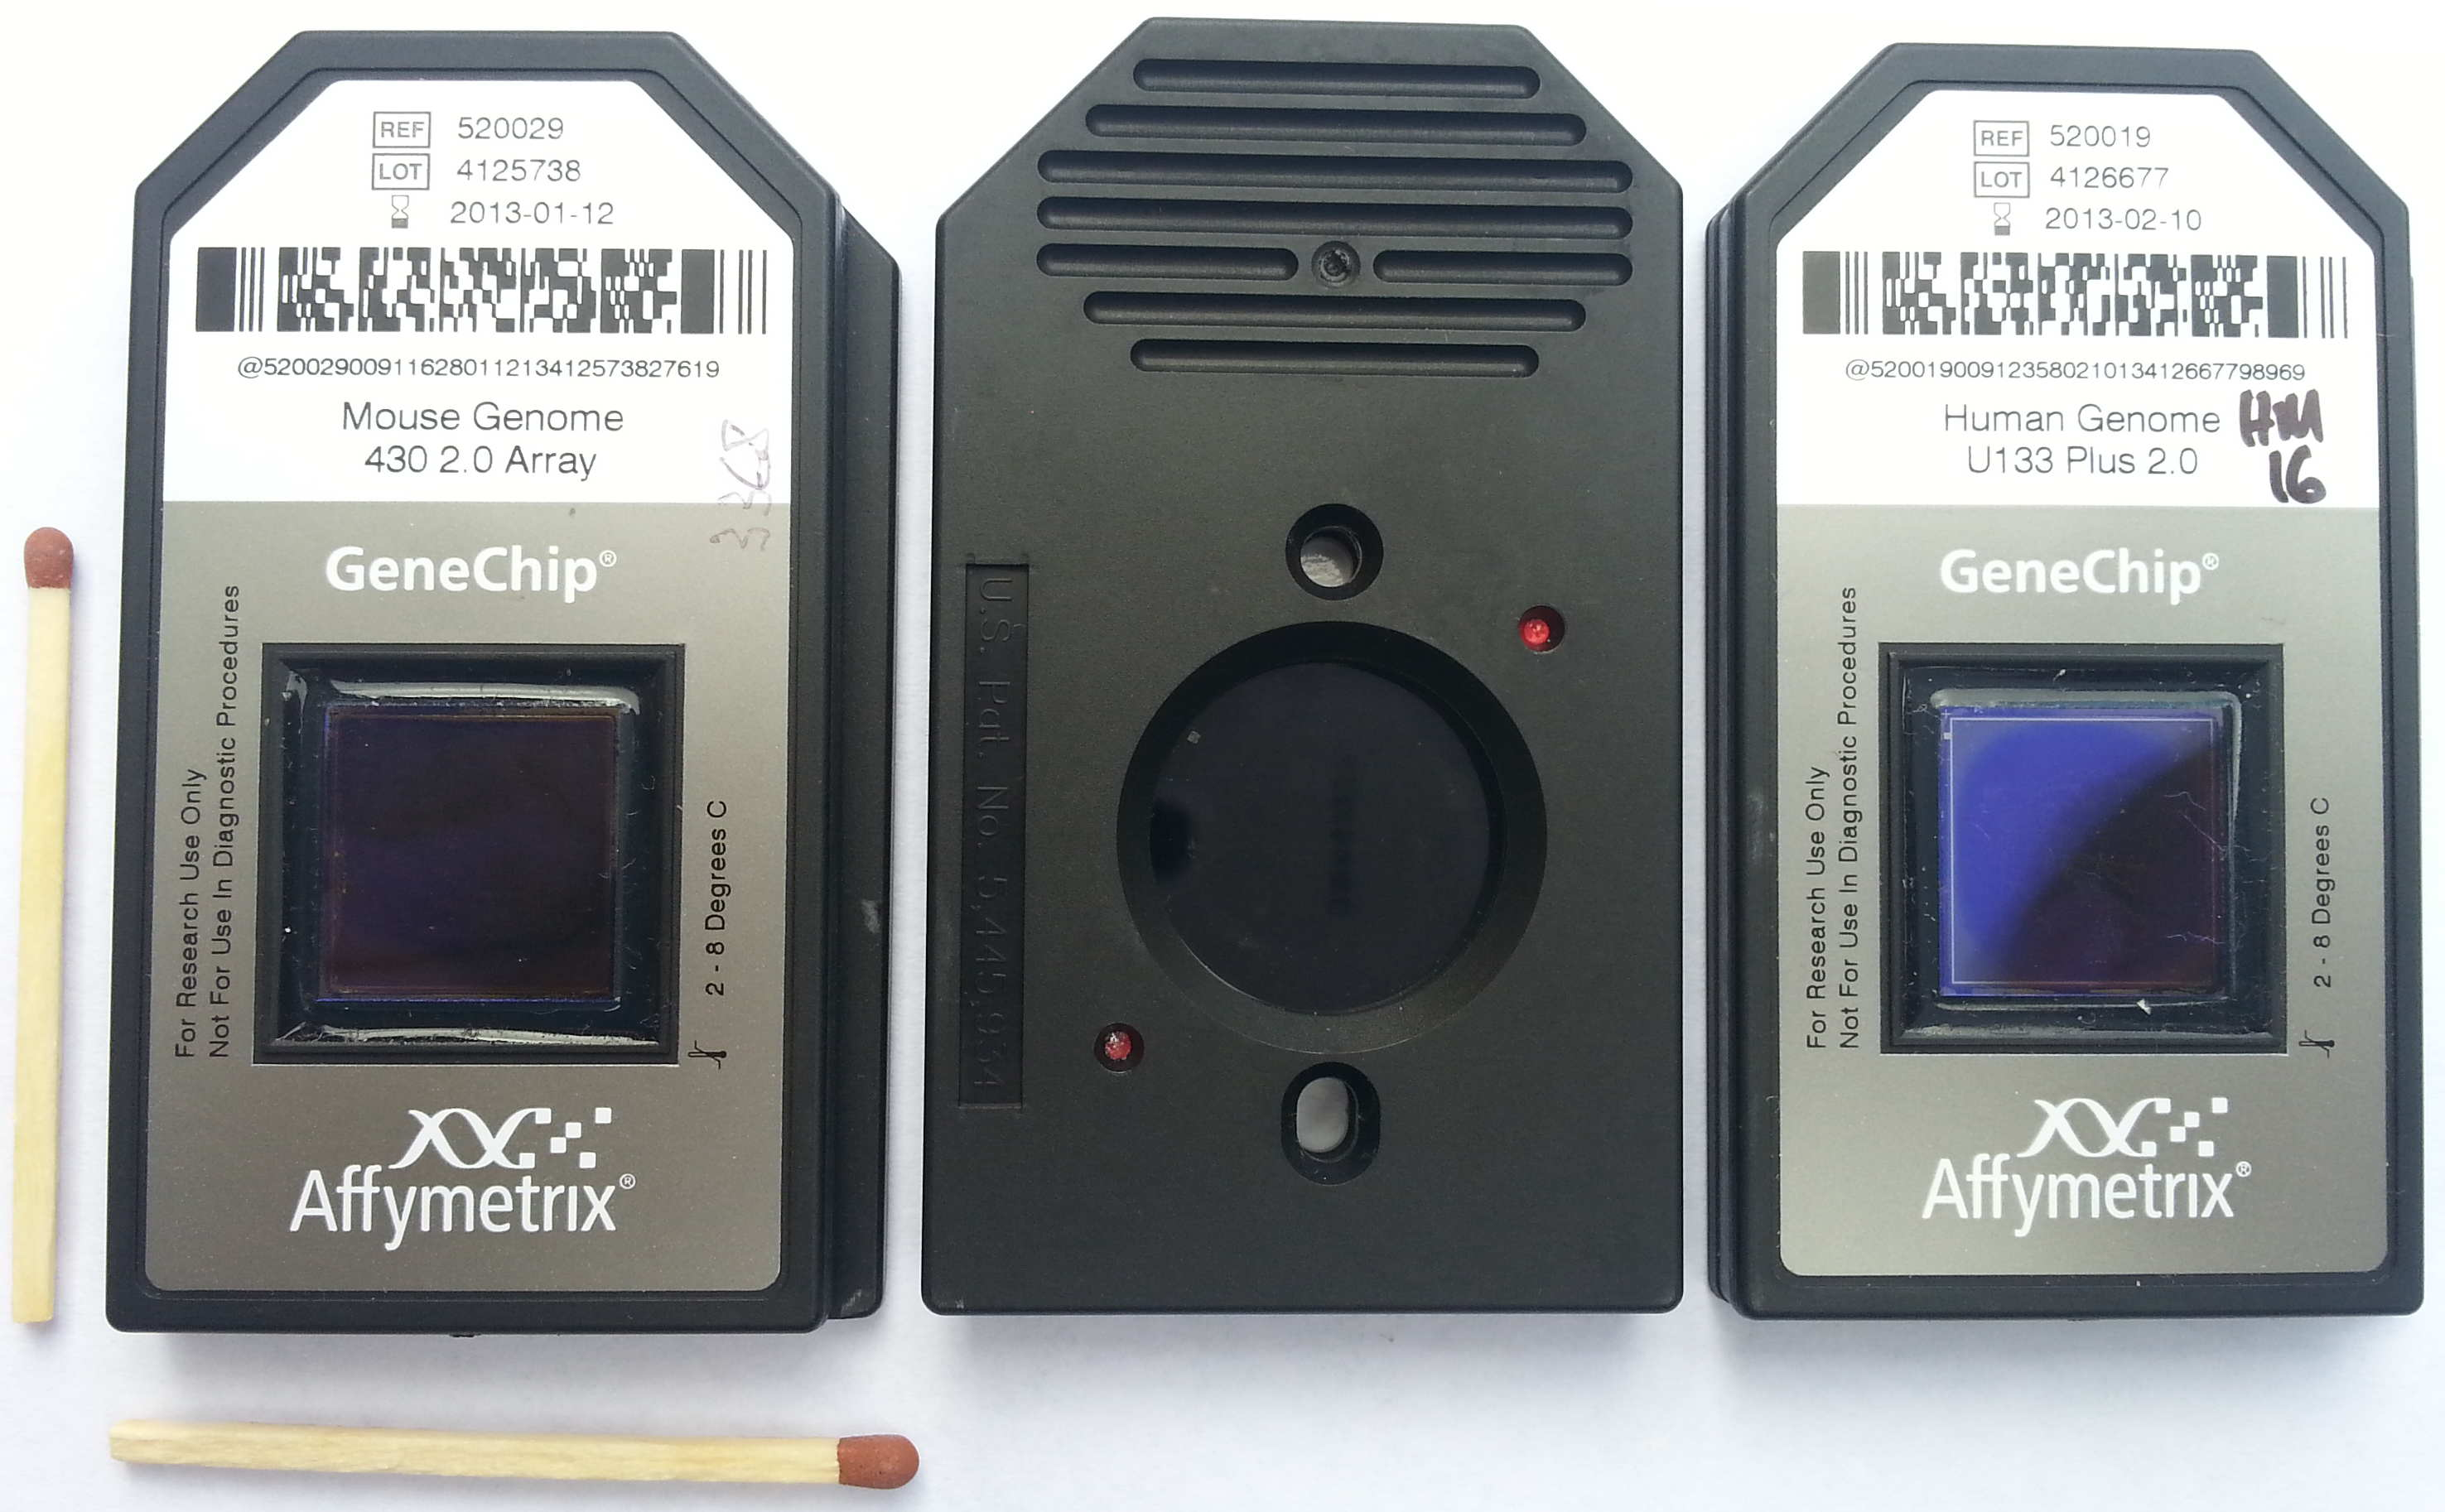
\includegraphics[width=.4\textwidth,keepaspectratio]{Affymetrix-microarray}
		\rule{35em}{0.5pt}
	\caption[Affymetrix Micro Array]{Gene Expression Data: Affymetrix Micro Array
	(Image courtesy Wikipedia. 
	\url{http://en.wikipedia.org/wiki/DNA_microarray})}
	\label{fig:Affymetrix-microarray}
\end{figure}
 
Figure \ref{fig:Affymetrix-microarray} shows two Affymetrix chips which contains DNA microarray. A match is shown at the bottom for the purpose of size reference of a microarray. The solid-phase DNA macroarray is usually a collection of ordered microscopic spots called features. Figure \ref{fig:Gene Expression Microarray} shows the schematic of the gene expression microarray data. On a typical Affymetrix microarray there are 6.5 million locations (represented by columns) with millions of identical DNA strands in every locations. Every strand construct with 25 probes or bases. 

The microarray is rinsed and washed with fluorescent stain. To accomplish a DNA test, two types of samples are used one is controlled sample and another is test sample. After extracting mRNA from DNA, copied are made from mRNA by reverse transcription. Two different fluorescent tagged with cyanide are usually used to differentiate between controlled samples and test samples. In general, green is used for controlled copy and red for test copy. Then the tagged samples are washed on the microarray. DNA is analysed based on matching with the probes on the microarray. A laser is used to glow the fluorescent molecules. After the hybridisation process a green spot represents a hybridisation with the controlled targets only, a red spot indicates hybridisation with the test targets only, yellow represent hybridisation both with the controlled targets and test targets, and black represents hybridisation with the neither samples, i.e. no hybridisation. Over the last couple of decades these gene expression data became one of the key resource of the biologists to diagnose diseases and drug discovery, gene discovery and determining genetic variations, aligning and comparing genetic codes, biomerker development, forensic application, functional analysis and also in the field of computational biology.

\cite{Ong:2002} modelled the regulatory pathway in E.coli from the time series gene expression microarray data by modelling causality, feedback loops or hidden variables using a Dynamic Bayesian network and tried to gain the insight of regulatory pathway. By analysing gene expression data \cite{Friedman:2000} were the first to determine the properties of transcriptional program for Baker's yeast using a Bayesian network.

\begin{figure}[t]
	\centering
	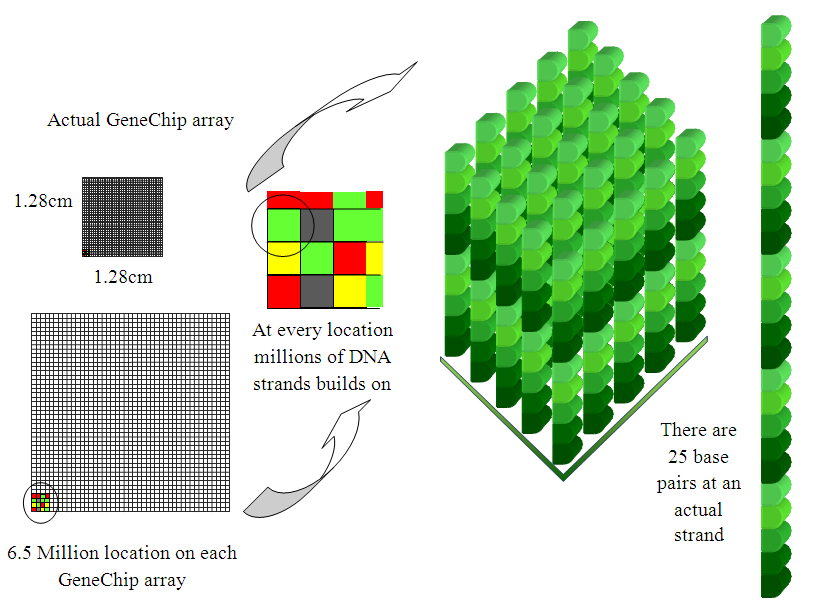
\includegraphics[width=\textwidth,keepaspectratio]{GeneExpressionMicroarray.png}
		\rule{35em}{0.5pt}
	\caption{Gene Expression Data: Affymetrix Micro Array}
	\label{fig:Gene Expression Microarray}
\end{figure}

Many of the recent studies already established the fact that the gene function of regulatory network depends on qualitative as well as quantitative aspects of the organisation of the network like high throughput data, including genomic sequence, expression profiles and transcription factor.

Among them one of the major challenges is to quantitative measurement and analysis of the mechanisms regulating mRNA transcription. Though using high throughput techniques it is comparatively easier to measure the output of transcription, but it is experimentally very complicated to measure the protein concentration levels of transcription factors and chemical affinity to the genes. Very often transcription factors are post-transcriptionally modified. So, the actual protein concentration levels and binding affinities could be an unreliable proxy of the mRNA expression levels of transcription factors (\cite{Sanguinetti:2006}).

Due to the advancement of the experimental technique lot of interest in recent years has been growing to infer information about regulatory activity from target genes. Now biologists can acquire the information about the structure of the transcriptional regulatory network. \cite{Lee:2002} determined the transcriptional regulatory network of yeast using chromatin immunoprecipitation(ChIP). They tried to figure out how yeast transcriptional regulators bind to promoter sequences across the genome. By calculating a confidence value (\textit{P} value) and setting up specific threshold they considered the protein-DNA interactions and artificially imposes a binding or not binding binary decision for each of the protein- DNA pair.

\subsection{\textit{Caenorhabditis elegans}}
\textit{Caenorhabditis elegans} is a nonparasitic, soil dwelling, small nematode worm. \textit{C. elegans} and other \textit{Caenorhabditis} species are found through all over the world. It can easily colonize mostly in the rotting materials with other microorganism. \textit{C. elegans} is easy to maintain in the petri dishes at the laboratory. At $25\,^{\circ}{\rm C}$ \textit{C. elegans} completeits life cycle in just 2.5 days from fertilized embryos to egg-laying adult through 4 larval stages. Its typical life span is 2-3 weeks. In 1965, Sydney Brenner introduced \textit{Caenorhabditis elegans} as a model organism to study the behaviour and development of animal (\cite{Brenner:1974}).

\begin{figure}%[htbp]
	\centering
		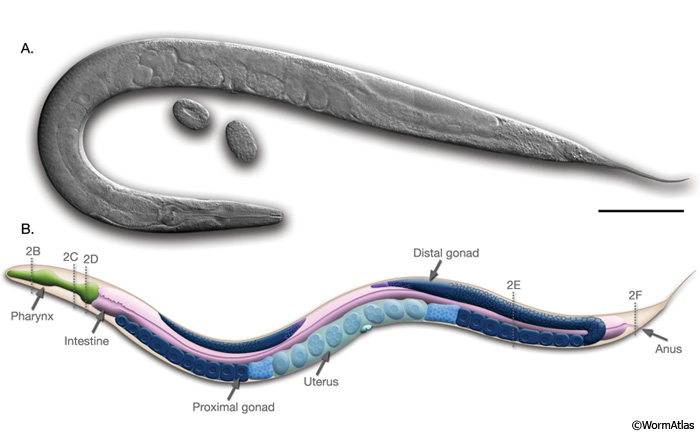
\includegraphics[width=8cm,keepaspectratio]{introfig1lr.jpg}
		\rule{35em}{0.5pt}
	\caption[Anatomy of an adult \textit{C.elegans}]{Anatomy of an adult hermaphrodite(\textit{C.elegans}). 
	A. DIC image of an adult hermaphrodite, left lateral side. Scale bar 0.1 mm. 
	B. Schematic drawing of anatomical structures, left lateral side 
	(Courtesy of WormAtlas \url{http://www.wormatlas.org/hermaphrodite/introduction/IMAGES/introfig1leg.htm}).}
	\label{fig:anatomy}
\end{figure}

\textit{C. elegans} is a relatively new addition as a model organism but its biological characteristics and property already been studied to an extraordinary level. The anatomical characteristics and detail development of this nematode was facilitated by its simple body plan. Its an eukaryote and it shares cellular and molecular structures and control pathways with higher organism. \textit{C. elegans}
is multicellular, an adult wild type  consist of 959 somatic cells and among these 302 are neurons (\cite{Sulston:1977, Palikaras:2013}). Its developmental process like embryogenesis, morphogenesis goes through a complex process to growth to an adult. Yet monitoring of the cellular process  and recording of cell division pattern is comparatively easier as its body is transparent. C Elegan's complete cell lineage at the electron microscopy level has been completed. Its already been established and this cell lineage is remarkably invariant between animal to animal (\cite{Brenner:1974, Byerly:1976, Sulston:1980, Wood:1988}).

To elucidate pathways and processes relevant to human biology and disease C. Elegans is using as a vital model. There are between $\sim20,250$ to $\sim21,700$ predicted protein-coding genes in \textit{C. elegans} (\cite{Gerstein:2010}). Using four different orthology-prediction methods \cite{Daniel:2011} assayed four methods to compile a list of \textit{C. elegans} orthologs of human genes. A  list of 7,663 unique protein-coding genes were resulted in that list and this represents $\sim38\%$ of the 20,250 protein-coding genes predicted in \textit{C. elegans}. When human genes introduced into \textit{C. elegans} human genes replaced their homologs. On the contrary, many \textit{C. elegans} genes can function with great deal of similarity to human like mammalian genes. So, the biological insight acquire from \textit{C. elegans} may be directly applicable to more complex organism like human.

\subsection{Transcription}
All the process in the body take places through some proteins. So, cells needs protein continuously. On the consequences, protein are required to be manufactured at every moment in the body. Inside cell protein is manufactured from the DNA. When any cells in the body is in need of protein, a special signal is sent to the DNA using hormones. Then proteins reside in DNA start to manufacture based on the received codes. The way that the enzymes finds the information required for protein construction is extremely complicated.

\begin{figure}%[tb]
	\centering
		 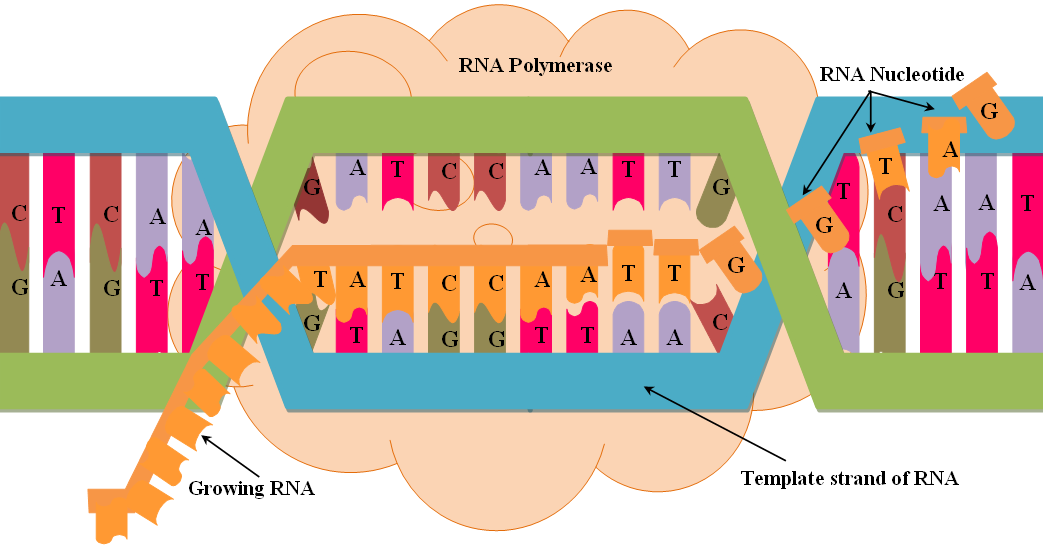
\includegraphics[width=0.7\textwidth,keepaspectratio]{Transcription.png} 
		\rule{35em}{0.5pt}
	\caption{A 'cartoon model' of DNA Transcription}
	\label{fig:transcription}
\end{figure}

DNA (Deoxyribonucleic acid) transcription is a process that involves the transcribing of genetic information from DNA to a complementary RNA (Ribonucleic acid). Protein is produced from the copy of DNA by the transcription process. This production of proteins and enzymes are controlled by the coding of cellular activity. Even the conversion of DNA to proteins is not straight forward. An RNA polymerase read the sequence of DNA, which produce an complementary RNA. DNA consists of four nucleotide bases named adenine (A), guanine (G), cytosine (C) and thymine (T) that are paired together (A-T and C-G) to give DNA its double helical shape. The major steps to the process of DNA transcription are :

\textbf{RNA polymerase binds to DNA:} In order to initiate the DNA transcription RNA polymerase and sigma factor form a holoenzyme. Transcription process starts at the promoter region of a double-stranded DNA. Sigma factor can recognize the DNA and its promoter region. \textbf{Elongation:} A sequence specific DNA binding factors called transcription factors then unwind the DNA strand. Elongation of the transcript then continues by the RNA polymerase and a sequence of chain is opened up. A messenger RNA (mRNA) is formed when RNA polymerase transcribe into a single stranded RNA polymer from a single strand of DNA.

\textbf{Termination:} RNA polymerase moves along the DNA unwinding its double helical form until it reaches the terminator sequence. At that point, RNA polymerase detaches from the DNA and releases the mRNA polymer. In this way DNA double helix is opened, transcribed and reclosed with minimum stress on the DNA molecule. At any certain time many RNA polymerase can transcribe a single DNA sequence, which can manufacture a large quantity of protein at once. 

\begin{figure}%[htbp]
	\centering
		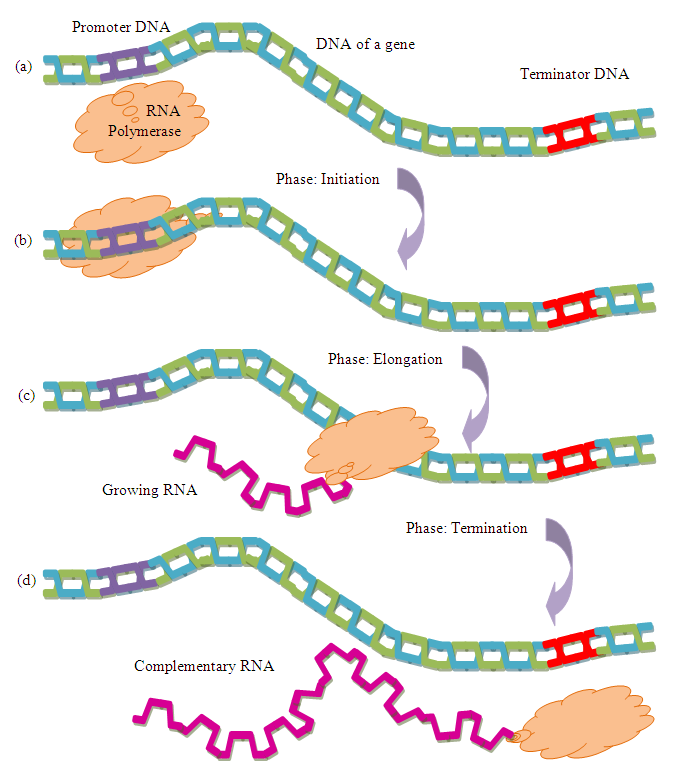
\includegraphics[scale=.6]{transcriptionProcess.png}
		\rule{35em}{0.5pt}
	\caption{A 'cartoon model' of Transcription Process: DNA Transcribed in mRNA}
	\label{fig:transcriptionProcess}
\end{figure}

\subsection{Transcription Factor}
A transcription factor is a protein that binds to DNA sequences and controls the flow of genetic information coding from DNA to mRNA (\cite{karin:1990, Latchman:1997}). Transcription factors can both promote or block the transcription process and act as an activator or repressor respectively (\cite{Lee:2000, Nikolov:1997, Roeder:1996}). A transcription factors may contain one or more DNA-binding domains. These binding domains attach to specific sequences of DNA adjacent to the genes that they regulate. Though some other protein such as coactivators, deacetylases, chromatin remodelers, kinases, histone acetylases, and methylases also play crucial roles in gene regulation but due to lack of DNA-binding domains they are not classified as transcription factors (\cite{Mitchell:1989, Ptashne:1997, Brivanlou:2002}). Figure \ref{fig:MappingEnvironmentalSignal} describes the mapping (we can also say ``cartoon'' mapping) between the environmental signal, transcription factors inside the cell, and the gene that they regulate. The environmental signal activates specific transcription factor proteins. After the activation the transcription factors bind DNA to change the transcription rate (the rate at which mRNA is produced) of 
specific target genes. The mRNA is then translated into protein by the process named translation (\cite{Alon:2006}). 

\begin{figure}%[]
	\centering
		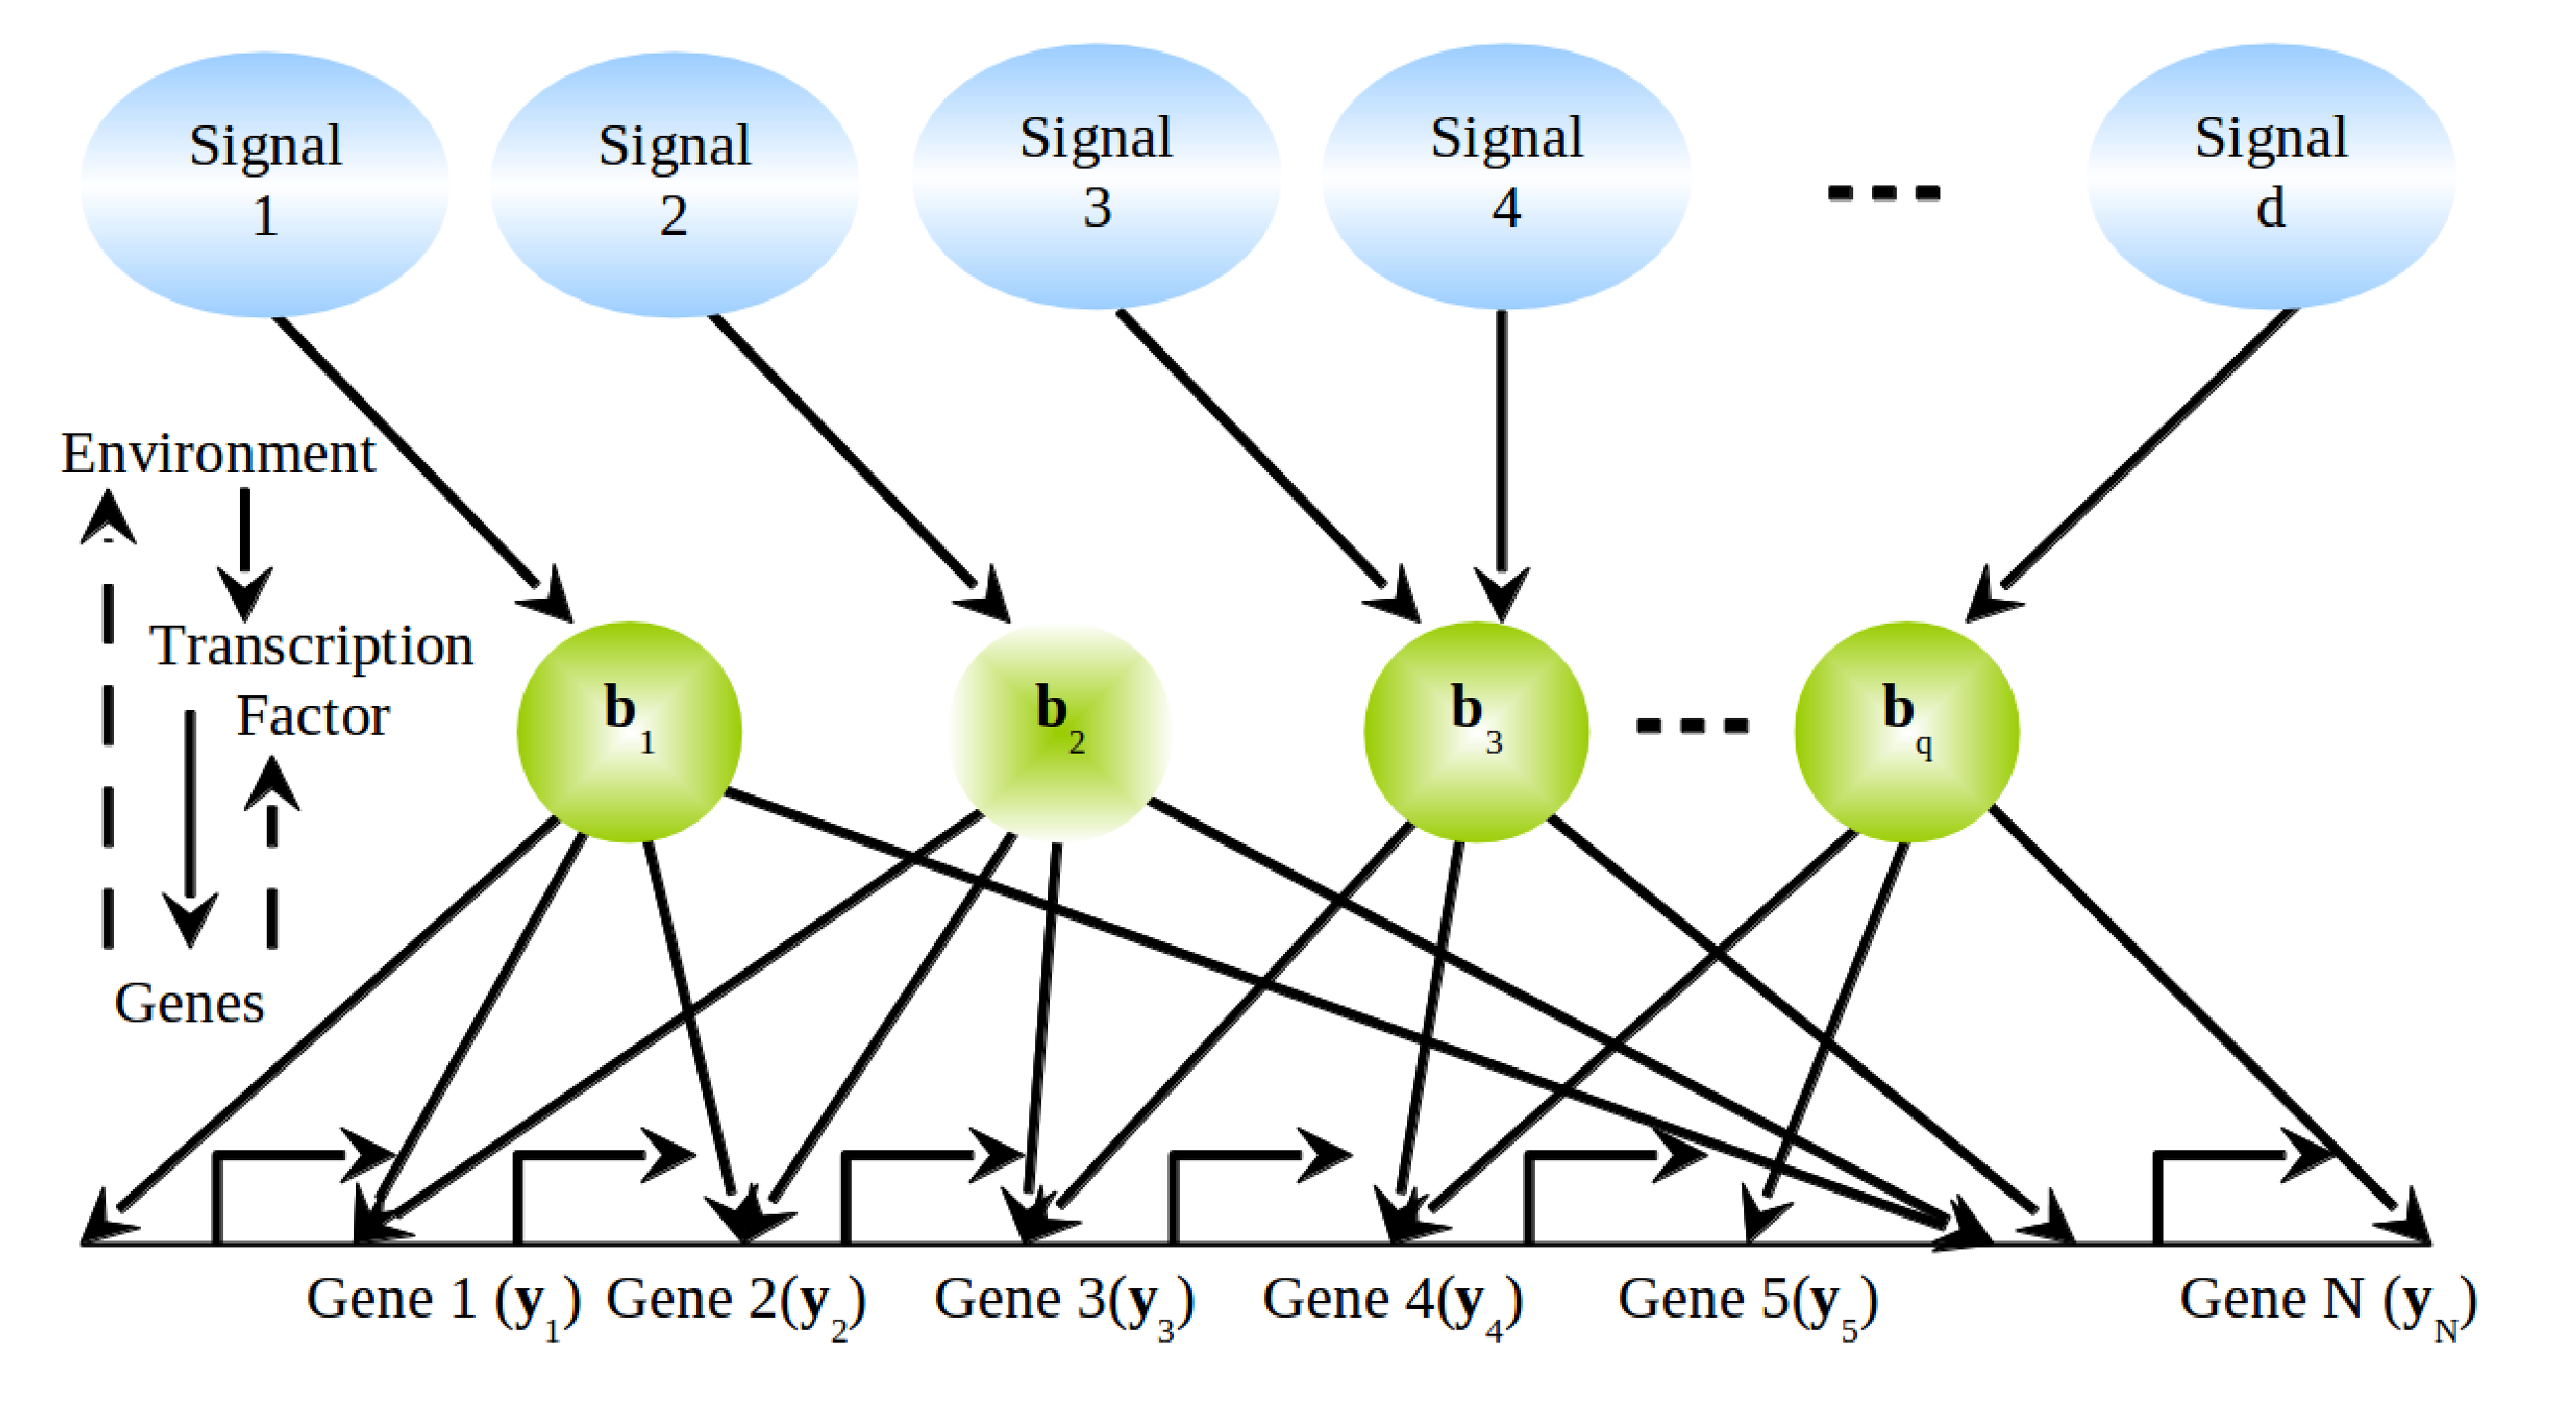
\includegraphics[width=\textwidth,keepaspectratio]{MappingEnvironmentalSignal.eps}
		\rule{35em}{0.5pt}
	\caption[The mapping between environmental signal, transcription factor 
	inside the cell the genes that they regulate]{The mapping between environmental signal, transcription factor 
	inside the cell the genes that they regulate (\cite{Alon:2006}).}
	\label{fig:MappingEnvironmentalSignal}
\end{figure}

\subsection{Amyotrophic lateral sclerosis and Mouse model}
Amyotrophic lateral sclerosis (ALS) also known as Lou Gehrig's disease or Motor neurone disease (MND) is a diverse neurodegenerative disorder. The median survival of this lethal disorder is less than 5 years! The disease is heterogeneous with variable severity in terms of speed of progression of the disease course. \cite{Brockington:2013, Peviani:2010}. From the view point biological aspect the disease progression speed is not clear yet. For experimental purpose many of the pathological and clinical features of human ALS can be replicated very well by transgenic mice. These murinae models also show the heterogeneity in the disease progression for the clinical phenotype. In a previous study \cite{Pizzasegola:2009} reported that disease progression is much faster in $129Sv$ than $C57$ mouse strain. Genomic analysis with gene expression time series data from these murinae models could be interesting to examine the the speed of propagation of ALS.

\section{Gaussian Processes}
Gaussian processes (GPs) are general class of models of functions. GPs are one of the most simple and widely used families of stochastic processes. As a general setting, Gaussian process of many types have been studied and incorporated in research for decades specially for modelling dependent data observed over time, or space, or time and space together. In GPs every observations in the input space are random variables from a Gaussian distribution. We included the introductory concepts of Gaussian process at Chapter \ref{ch:GaussianProcessRegression}.
%TODO

\section{Summary of the main goal of the thesis}
We will set some generic goals for this thesis and later we will try to achieve them chronologically:

\textbf{Generic goal 1}: We will aim to develop a tool (with programming language $R$) using probabilistic model for transcription factor activities. To step forward from a unicellular microorganism (e.g.\ yeast) to a multicellular eukaryote (e.g.\ \textit{C.elegans}) we will build the connectivity information and analyse the transcription factor activities using our tool.

\textbf{Generic goal 2}: We will target to find an pathway to overcome the limitation of the parametric Markovian assumption based linear Gaussian model to non-parametric Gaussian process with a particular 
covariance function.

\textbf{Generic goal 3}: We will design a kernel or covariance function of Gaussian process to model the dynamic behaviour of transcription factors for given gene expression time series data and connectivity information between genes and transcription factors.

\textbf{Generic goal 4}: Our final goal of this thesis is to develop a new clustering method based on hierarchy of Gaussian processes to model condition-specific and gene-specific temporal covariances which allows each cluster to be parametrised according to whether the behaviour of the genes across conditions is correlated or anti-correlated. 

\section{Road Map}
The thesis is structured in the following chapters:

\textbf{Chapter 1}: This documents starts with some basic concepts and general terminology to the field of interest to addressed some key issues which will be tackled or achieved later on this work.

\textbf{Chapter 2}: This chapter starts with the basis concepts of probabilistic model. After describing the connectivity information between genes and transcription factors we briefly describe the probabilistic model for transcription factor activities. Earlier this problem was solved for a unicellular microorganism (yeast) but we have forwarded the mathematical model of transcription factors activates for a multicellular eukaryote (\textit{C.elegans}) building our own connectivity information.
 
\textbf{Chapter 3}:
This is a technical background chapter where we briefly describe Gaussian process, regression problem and regression with Gaussian process. Choosing an appropriate kernel is one of the key issue while modelling with Gaussian process. In this chapter we briefly describe about some commonly used kernels. We also mentioned about hyperparameter learning. Why and which kernel could be an appropriate choice while modelling the transcription factor activity using Gaussian process was justified at the later section of this chapter.

\textbf{Chapter 4}:
We note that the linear Gaussian model is equivalent to a Gaussian process with a particular covariance function. We therefore build a model directly from the Gaussian process perspective to achieve the same 
effect. In this chapter we design a covariance function for reconstructing transcription factor activities given gene expression profiles and a connectivity information between genes and transcription factors. We introduce a computational trick, based on  judicious application of singular value decomposition, to enable us to efficiently fit the Gaussian process in a reduced 'TF activity' space. 

\textbf{Chapter 5}:
Amyotrophic lateral sclerosis is an irreversible neurodegenerative disorder that kills the motor neurons and results in death within 2 to 3 years from the symptom onset.  Speed of progression for different patients are heterogeneous with significant variability. Transgenic mice from different backgrounds showed consistent phenotypic differences for disease progression. We used a hierarchy of Gaussian processes to model condition-specific and gene-specific temporal covariances. In this chapter we develop a new clustering method that allows each cluster to be parametrised according to whether the behaviour of the genes across conditions is correlated or anti-correlated. By specifying correlation between such genes we gain more information within the cluster about how the genes interrelate. This chapter also includes the gene enrichment score analysis and KEGG pathway analysis that we used on our clustering analysis results for biological validation.

\textbf{Chapter 6}
The final chapter concludes this thesis by summarising the achievements highlighting its novelties. It also raises some important questions that need to be considered in the future.

% \section{Publication related with this thesis}
% 
% %TODO

\section{Notation, Symbols and Acronyms}

%TODO

\section*{Acronyms}
\begin{acronym}
\acro{cDNA}{Complementary Deoxyribonucleic Acid}
\acro{C.elegans}{Caenorhabditis elegans} 
\acro{ChIP}{Chromatin Immunoprecipitation} 
\acro{DIC}{Differential Interference Contrast} 
\acro{DNA}{Deoxyribonucleic Acid} 
\acro{EDGEdb}{C. elegans Differential Gene Expression Database} 
\acro{GP}{Gaussian process} 
\acro{GPLVM}{Gaussian process Latent Variable Model} 
\acro{GPy}{a Gaussian processes framework in python} 
\acro{KEGG}{Kyoto Encyclopedia of Genes and Genomes}
\acro{LLS}{Log Likelihood Score} 
\acro{LVM}{Latent Variable Model} 
\acro{mRNA}{messenger Transfer Ribonucleic Acid} 
\acro{PCA}{Principal Component Analysis}
\acro{PLS}{Partial Least Square} 
\acro{PPCA}{Probabilistic Principal Component Analysis}
\acro{RBF}{Radial Basis Function} 
\acro{RNA}{Ribonucleic Acid}
\acro{RT-PCR}{Reverse Transcription Polymerase Chain Reaction}  %TODO check
\acro{SE}{Squared Exponential} 
\acro{SVD}{Singular Value Decomposition} 
\acro{TF}{Transcription Factor} 
\acro{TFA}{Transcription Factor Activity}  
\end{acronym}